
\subsection{Deceleration Parameter}
We conclude our overview of cosmology with one final perspective, the Universe as seen through the deceleration parameter.  The deceleration parameter is another indicator of the transition between different eras of the Universe's history.  Recall the relation \req{qparam} (for $k=0$)  between deceleration parameter and matter content of the Universe. In particular we have the regimes

\begin{itemize}
\item Radiation dominated Universe: $P=\rho/3 \implies q=1$.\\


\item  (Non-relativistic) Matter dominated Universe: $P\ll\rho \implies q=1/2$.\\



\item Dark energy ($\Lambda$) dominated Universe: $P=-\rho \implies q=-1$.\\

\end{itemize}
We use $q$ first to characterize the era from today back to the end of neutrino freeze-out and then from freeze-out until the end of the hadron era.


%%%%%%%%%%%%%%%%%%%%%%%%%%%%%%%%%%%%%%%%%%%%%%%%%%%%%%%%%%%%%%%
\subsubsection{Back in time to Neutrino Freeze-out}\label{recomb}
In the following we use the mix of matter  (31\%) and dark energy (69\%) with photon and neutrino backgrounds favored by the latest Planck results \cite{Planck}, where we gave two neutrino species mass of $m_\nu=30\meV$ and a third neutrino remains  massless.  This is a different mass value than used above and again, it is only for illustration-- other mass choices are possible within present day constraints and will impact to some degree where exactly matter dominance emerges from the radiative Universe.  We presume  that neutrino kinetic freeze-out completed before the onset of $e^\pm$-annihilation into  photons, leading to the neutrino to photon temperature ratio \req{T_nu_T_gamma}. Again, this is a common simplifying assumption.  Much of the remainder of this work will involve improving on this approximation, but for the purposes of this overview it is sufficient.

Figure \ref{fig:today} shows in the left frame the temperature  (left axis) and deceleration parameter (right axis)  from shortly after the completion neutrino freeze-out until today.  The horizontal dot-dashed lines show  the pure radiation-dominated value of $q=1$ and the matter-dominated value of $q=1/2$. The expansion in this era starts off as radiation-dominated, but transitions to matter-dominated starting around $T=\mathcal{O}(10\eV)$ and begins to transition to a dark energy dominated era at $T=\mathcal{O}(1\meV)$. We are still in the midst of this transition today. The vertical dot-dashed lines show  the time of recombination at $T\simeq0.25\eV$, when the Universe became transparent to photons, and reionization at $T\simeq {\cal O}(1\meV)$, when hydrogen in the Universe was again ionized due to light from the first galaxies \cite{Zaroubi:2012in}. 

On the right in figure  \ref{fig:today}  we show the Hubble parameter $H$ and redshift $z+1\equiv a_0/a(t)$. We can see in figure \ref{fig:today} a visible deviation from power law behavior due to the transitions from radiation to matter dominated and from matter to dark energy dominated expansion.  These transitions are accentuated and more easily visualized in the form of the deceleration parameter $q$. The time span covered by the figure  \ref{fig:today} is in essence the entire lifespan of the Universe, but of course on a logarithmic time scale there is a lot of room for interesting physics in the tiny blip that happened beforehand.


%%%%%%%%%%%%%%%%%%%%%%%%%%%%%%%%%%%%%%%
\begin{figure}
\begin{minipage}{\linewidth}
\makebox[0.5\linewidth]%
{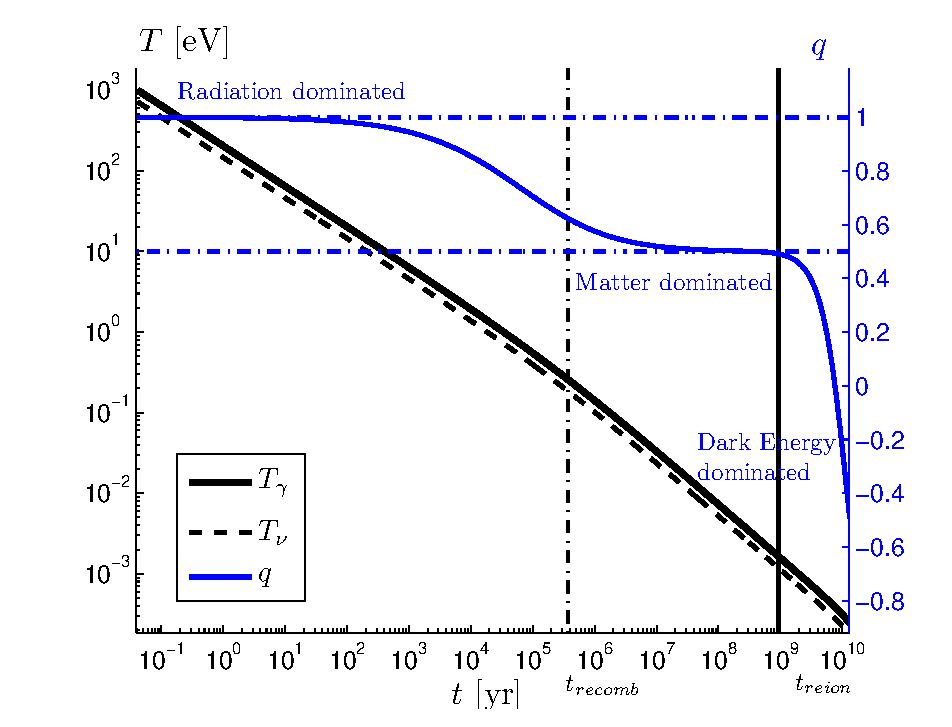
\includegraphics[keepaspectratio=true,scale=0.52]{03-birrell/ErasOfUniverse/T_q_today.eps}}
\makebox[0.5\linewidth]%
{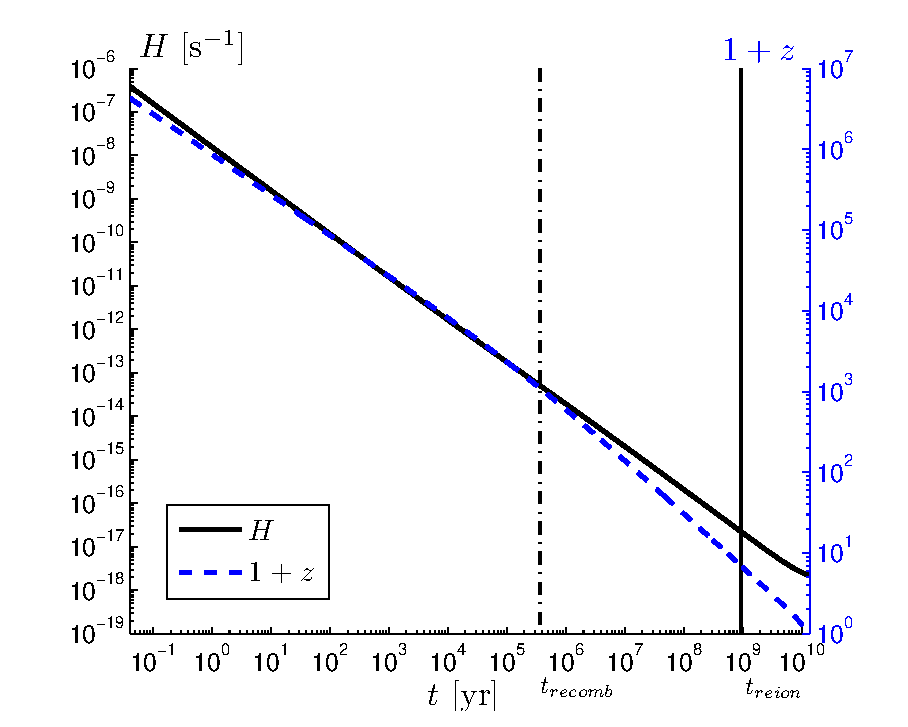
\includegraphics[keepaspectratio=true,scale=0.52]{03-birrell/ErasOfUniverse/H_z_today.eps}}
\caption{Transition periods in the composition of the Universe: on left -- evolution of temperature $T$  and deceleration parameter $q$; on right --  evolution of the Hubble parameter $H$ and redshift $z$.
\label{fig:today} }
\end{minipage}
\end{figure}
%%%%%%%%%%%%%%%%%%%%%%%%%%%%%%%%%%%%%%%

%%%%%%%%%%%%%%%%%%%%%%%%%%%%%%%%%%%%%%%%%%%%%%%%%%%%%%%%%%%%%%%
\subsubsection{Neutrino Freeze-out Era }\label{nudecoup}
%%%%%%%%%%%%%%%%%%%%%%%%%%%%%%%
The era separating the photon-neutrino-matter-dark energy Universe we just described from the end of the hadron Universe is quite complex in its evolution.   We begin when the number of $e^\pm$-pairs has decayed to the same abundance as the number of baryons in the Universe at the temperature  $T=\mathcal{O}(10\keV)$ and reach back to $T={\cal O}(30\MeV)$ where muons and pions are disappearing from the Universe.

%%%%%%%%%%%%%%%%%%%%%%%%%%%%%%%%%%%%%%%
\begin{figure}
\begin{minipage}{\linewidth}
\makebox[0.5\linewidth]%
{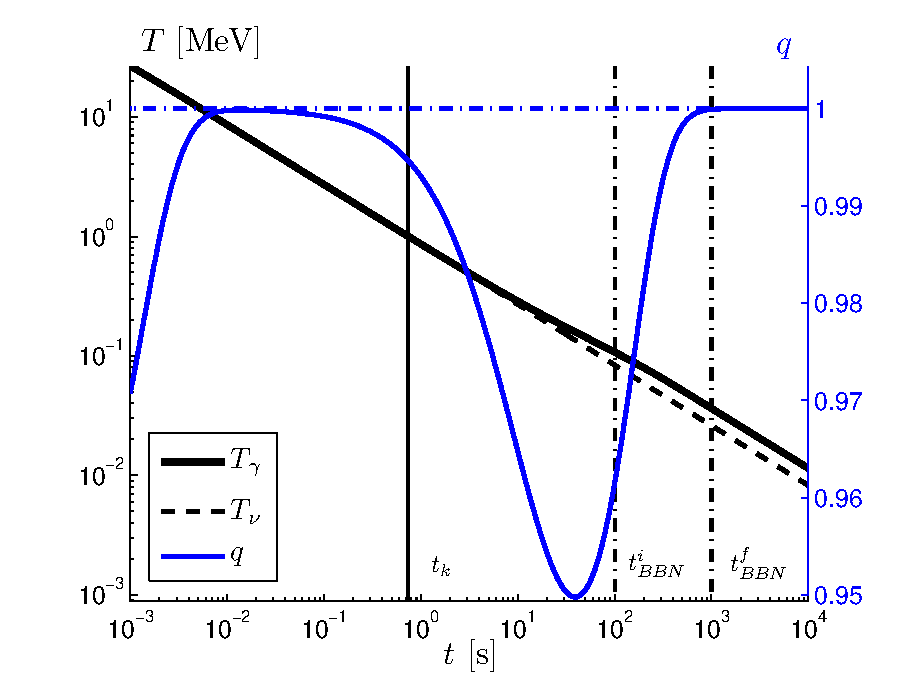
\includegraphics[keepaspectratio=true,scale=0.54]{03-birrell/ErasOfUniverse/T_q_BBN.eps}} 
\makebox[0.5\linewidth]%
{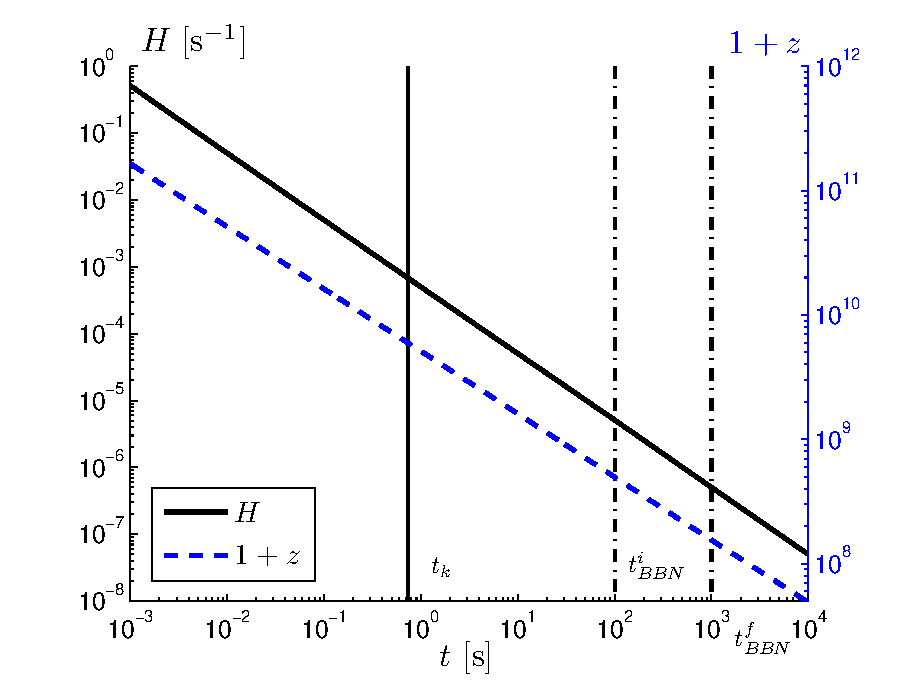
\includegraphics[keepaspectratio=true,scale=0.54]{03-birrell/ErasOfUniverse/H_z_BBN.eps}} 
\caption{From the end of baryon antimatter annihilation through BBN, see figure \ref{fig:today}.%  on left -- evolution of temperature $T$  and deceleration parameter $q$; on right --  evolution of the Hubble parameter $H$ and redshift $z$.
\label{fig:BBN}  }
\end{minipage}
\end{figure}
%%%%%%%%%%%%%%%%%%%%%%%%%%%%%%%%%%%%%%%

 In figure~\ref{fig:BBN} the horizontal dot-dashed line for $q=1$  shows the pure radiation dominated value with two exceptions. First, the presence of massive pions  and muons reduce  the value of $q$ near to the maximal temperature shown.  Second, when the temperature is near the value of the electron mass, the $e^\pm$-pairs are not yet fully depleted but already sufficiently non-relativistic to cause another dip in $q$.  These are not large drops; the expansion is still predominately radiation dominated.  But $q$ provides a sensitive measure of when various mass scales become relevant and is a good indicator of the presence of a reheating period.

 The dashed line shows the neutrino temperature, which decouples from the $e^\pm$ and photon temperature at $T={\cal O}(1\MeV)$ when neutrinos freeze-out and begin free streaming. In figure~\ref{fig:BBN} the unit of time is seconds and the range spans the domain from fractions of a millisecond to a few hours. After neutrino freeze-out we come to Big Bang Nucleosynthesis, the period when the lighter elements were synthesized in a hot but relatively dilute plasma \cite{Iocco:2008va}. We left some time gap between this and the domain shown in figure \ref{fig:today}  describing the current era -- there is an uneventful evolution between the two domains. 

\subsection{Focusing on Neutrino Freeze-out}
Neutrino freeze-out is, as far as we know, the unique era in the history of the Universe when a significant matter fraction froze out at the same time that a reheating period was beginning, namely the start of $e^\pm$ annihilation.  It is this coincidence that makes neutrino freeze-out a rich and complicated period to study as compared to the many other reheating periods in the history of the Universe. This period has been studied before \cite{Madsen,Dolgov_Hansen,Gnedin,Esposito2000,Mangano2002,Mangano2005}, but the Planck satellite results \cite{Planck} motivate a reinvestigation of this period of cosmology.  We therefore make the interplay of neutrino freeze-out and reheating from $e^\pm$ annihilation the primary focus of the remainder of this work.

\subsection{Conventions}\label{app:conventions}
There are several sign conventions in use in general relativity.  As discussed in \cite{hobson}, these conventions differ by the sign factors $S1$, $S2$, $S3$, which appear in the following objects:
\vspace{3mm}

Metric Signature: $\eta^{\mu\nu}=(S1)\text{Diag}(-1,1,1,1)$
\vspace{3mm}

Riemann Tensor: $R^\mu_{\alpha\beta\gamma}=(S2)(\partial_{\beta}\Gamma^\mu_{\alpha\gamma}-\partial_{\gamma}\Gamma^\mu_{\alpha\beta}+\Gamma^\mu_{\sigma\beta}\Gamma^\sigma_{\gamma\alpha}-\Gamma^\mu_{\sigma\gamma}\Gamma^\sigma_{\beta\alpha})$
\vspace{3mm}

Einstein Equation: $G_{\mu\nu}-(S3)\Lambda g_{\mu\nu}=(S3)8\pi G_NT_{\mu\nu}$
\vspace{3mm}

Ricci Tensor: $R_{\mu\nu}=(S2)(S3)R^\alpha_{\mu\alpha\nu}$
\vspace{3mm}

The sign $S3$ comes from the choice of what index is contracted in forming the Ricci tensor.  Since that sign factor appears in both $R_{\mu\nu}$ and $R$ it affects the overall sign of $G_{\mu\nu}$ and therefore Einstein's equation as shown above. In this dissertation we will use the $(-,+,-)$ convention.



